\section{Introduction}
For repository-level coding tasks such as those in the popular SWE-Bench benchmark \citep{jimenez2024swebenchlanguagemodelsresolve}, a critical first step is \textbf{code localization}: given an issue description and a codebase, the system must identify the relevant files and finer-grained code entities (e.g., classes and functions) to modify~(\S\ref{sec:background}; \citet{husain2019codesearchnet,xia2024agentless}).
This is challenging in large repositories with complex inter-dependencies, and relying on general-purpose language models to solve this localization problem as part of the agentic coding loop can result in high costs, incorrect fixes, and code bloat~\citep{hong2025context}.

To address this issue, it is also common to incorporate some variety of specialized localization module to acquire the relevant context from large codebases in a more efficient and effective manner.
Traditionally, this code search was performed through semantic code search using vector databases \citep{xia2024agentless,wang2025coderag}. In contrast, recent methods have investigated \emph{agentic code search} - using agents to iteratively navigate the repository and uncover necessary evidence for solving the issue under consideration.
Typically, these methods have involved significant modifications to the agent itself to incorporate static analysis of the codebase, such as LocAgent's repository graph navigation \citep{chen-etal-2025-locagent} and RepoNavigator's ``jump'' tool that retrieves definitions of Python symbols \citep{zhang2025one}.
While well-grounded, these necessitate the use of static analysis tools tailored to a \emph{particular} programming language, increasing operational complexity of deploying such agents on a broader variety of coding scenarios.
Simultaneously, there have been various anecdotal reports from industry regarding reinforcement learning methods that increase the ability of agents to perform localization rapidly \citep{cognition2025swegrep,cursor2025composer}, with varying levels of detail but without a clear training recipe.
\begin{figure*}[!ht]
    \centering
    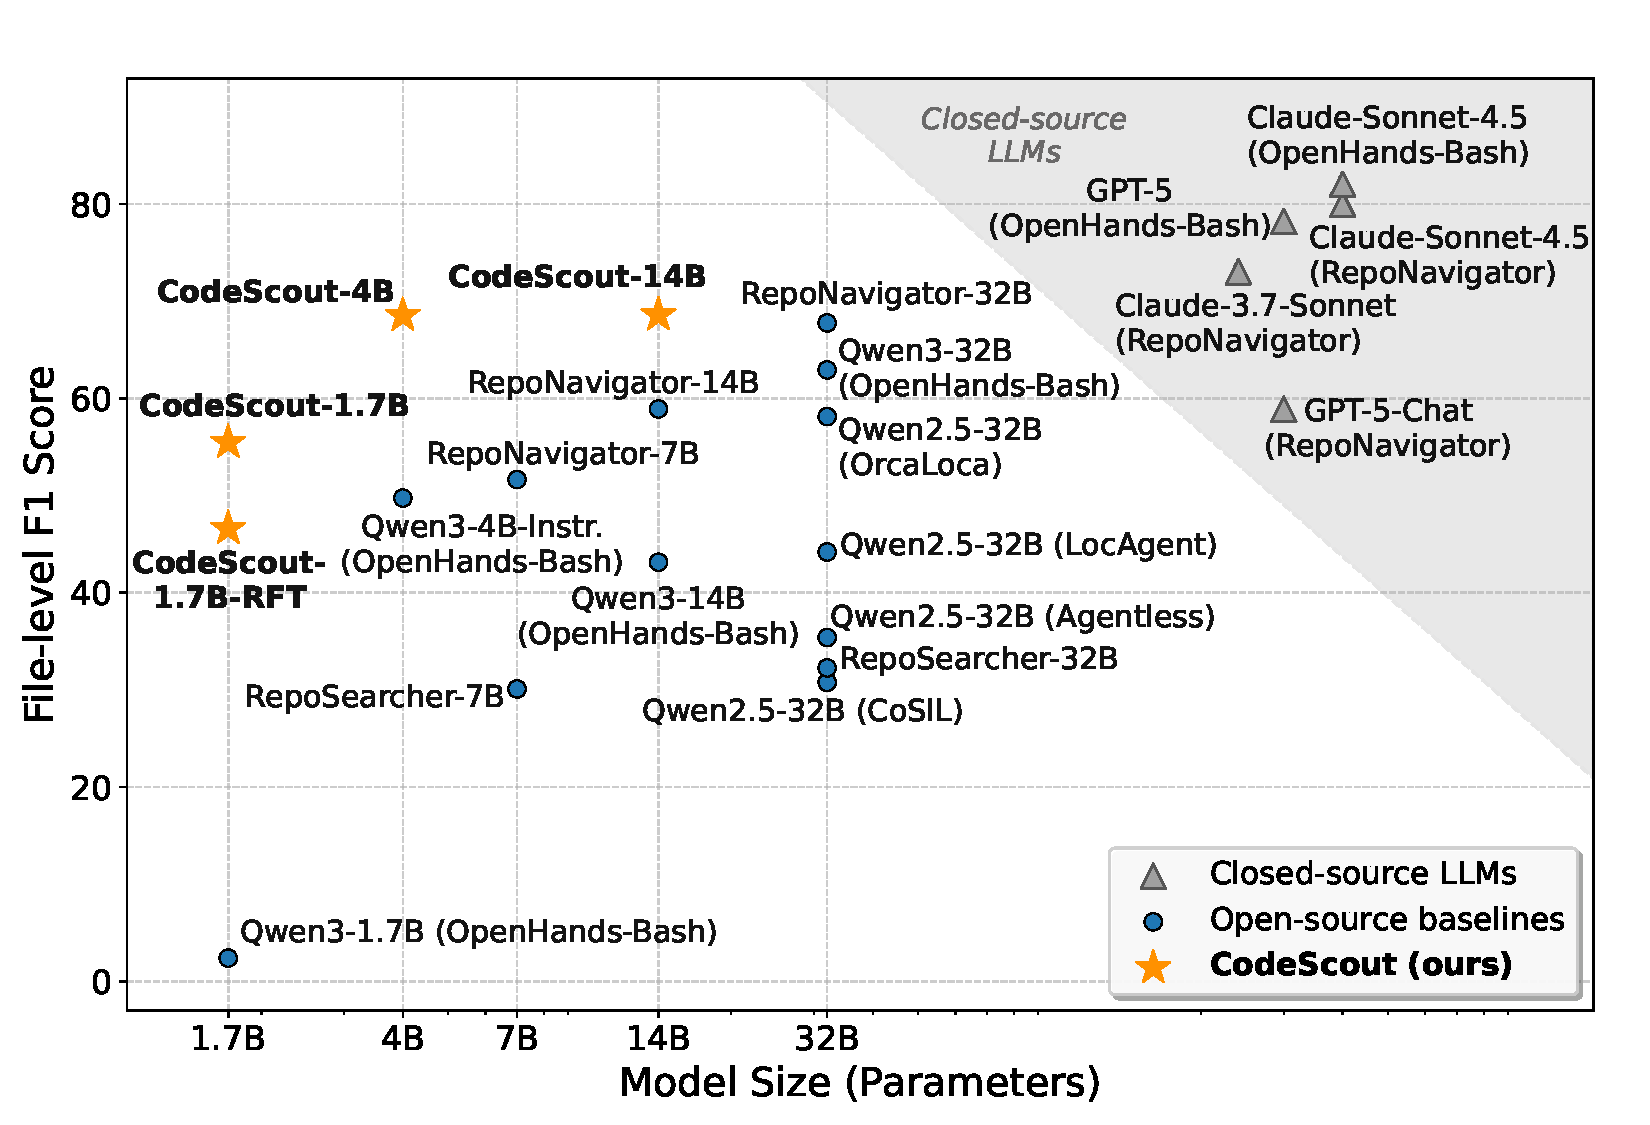
\includegraphics[width=0.49\columnwidth]{COLM/Figures/f1_vs_params_verified_file_new.pdf}
    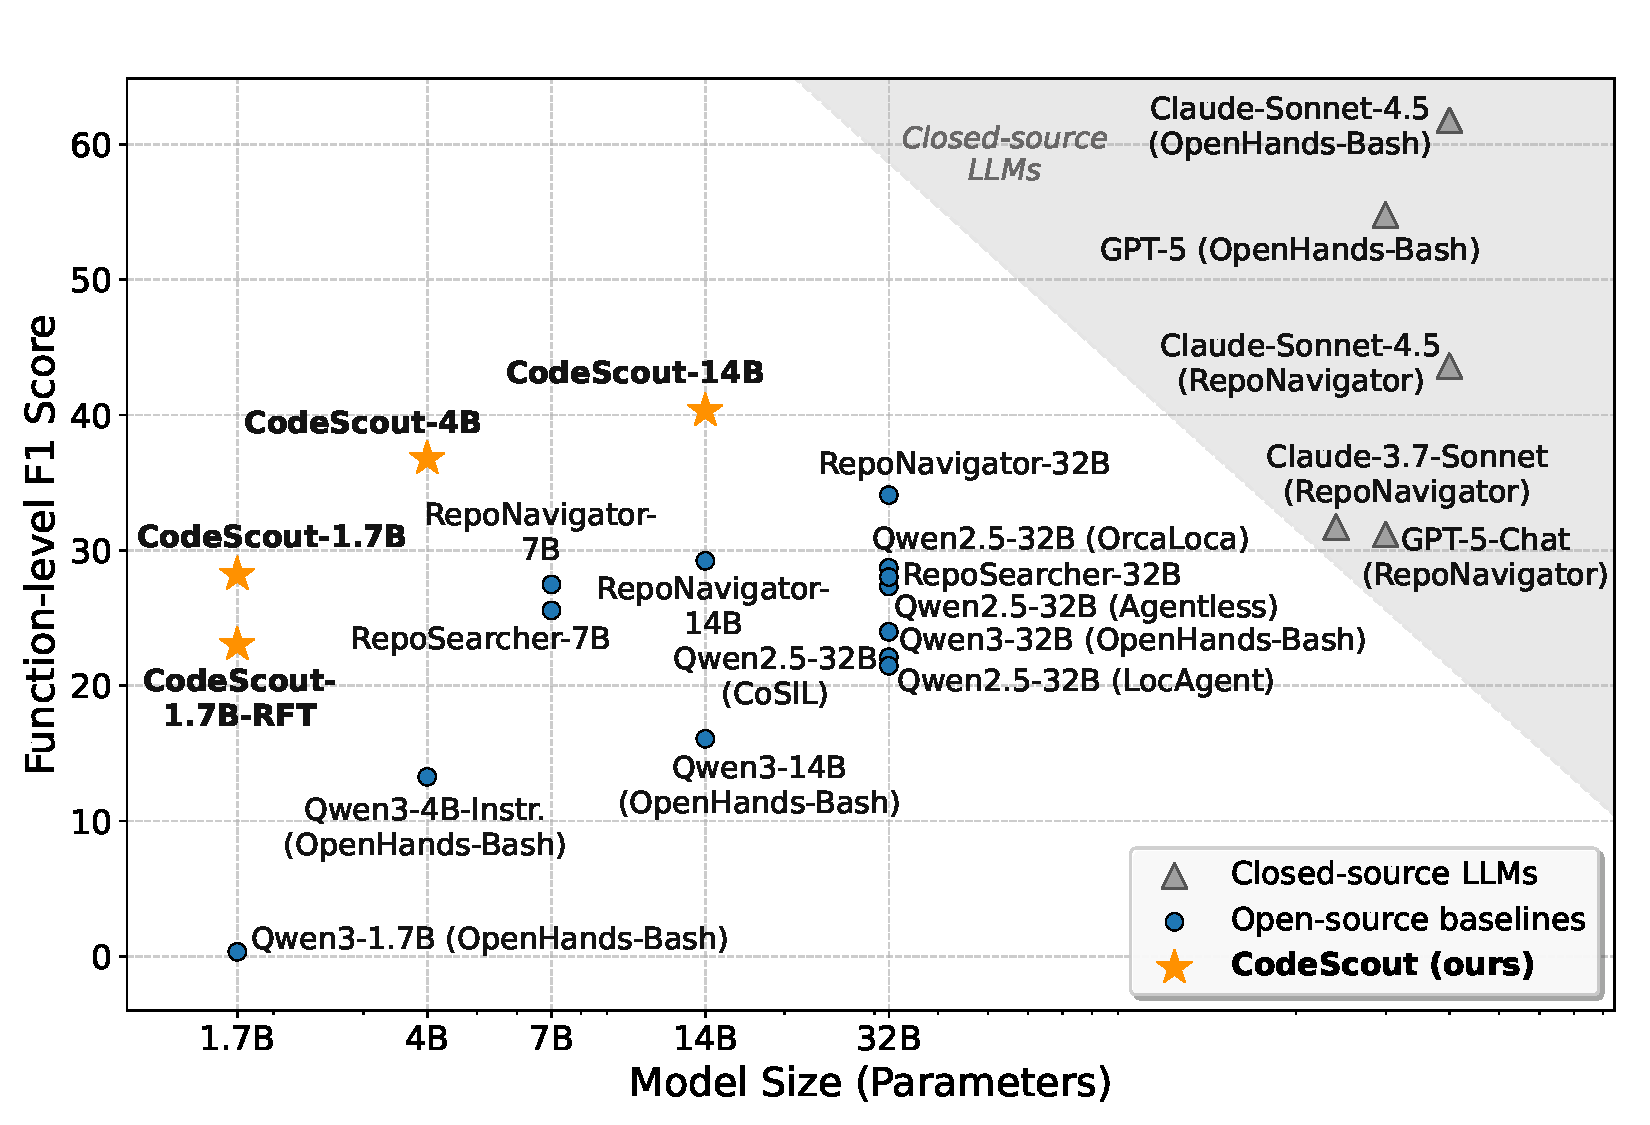
\includegraphics[width=0.49\columnwidth]{COLM/Figures/f1_vs_params_verified_function_new.pdf}
    \caption{An overview of code localization performance of various approaches on SWE-Bench Verified. \methodname achieves superior or competitive results over larger SoTA open-source LLMs and closes the gap with frontier closed-source LLMs.}
    \label{fig:main}
\end{figure*}
Given this background, we address the fundamental research question: \emph{given an appropriate reinforcement learning algorithm, what is an effective recipe to train a code localization agent that simply uses the terminal tool typical of more generic coding agents, yet achieves competitive or superior accuracy over agents using special-purpose tools?}
This work provides the first public demonstration of such a recipe, which involves scalable methods for data and environment creation (\S\ref{sec:data_creation}), a standard agent scaffold (\S\ref{sec:agent_scaffold}), careful attention to reward design (\S\ref{sec:reward_design}) and training algorithm (\S\ref{sec:train_algo}).
In experiments (\S\ref{sec:experiments}, \S\ref{sec:results}), we find that the resulting model \methodname achieves localization performance superior to or competitive with existing methods on a variety of localization datasets derived from SWE-Bench Verified, Pro, and Lite. Importantly, all models and code are released publicly, building a strong baseline for future research to build upon.
% \sonicomment{Do we need to explicitly create a bulleted list of research contributions with 3 points as done by some papers?}
% \gncomment{No, these are often repetitive and unnecessary}
% \sonicomment{Ok sir, thanks!}

% To address this inefficiency, the community has begun exploring specialized \textbf{localization} subagents that identify relevant code before handing off to a downstream code editing agent, rather than relying on a monolithic agent to perform both search and editing~\citep{zhang2026toolenoughreinforcementlearning}.

% Despite these advances, most high-performing code localization systems remain closed-source. Some open-source alternatives (e.g., LocAgent~\citep{chen-etal-2025-locagent}) use proprietary API trajectories (e.g., Claude-3.5) for distillation, which can limit reproducibility and deployment in privacy-sensitive settings. RepoNavigator~\citep{zhang2026toolenoughreinforcementlearning} demonstrates RL training without distillation for repository-level agents; in contrast, we focus on training a dedicated localization subagent with a lightweight tool scaffold and multi-level F1 rewards.

% In this work, we present \textbf{an open-source recipe for training dedicated code localization agents using reinforcement learning}. Our contributions are three-fold: \yccomment{To be refined later.}
% \sonicomment{We should add some summary of the results here saying that our training recipe is outperforming closed-source models + complex scaffolds, and even 8x larger models on Pro/Verified/Lite}
% \yccomment{Agreed. I’ll revise this after the details done; and please flag any inaccuracies.}
% \begin{enumerate}
%     \item \textbf{Multi-level localization with RL training}: We formulate code localization as multi-level target prediction at three granularities (file, class, and function), and optimize multi-level F1 rewards. We train \methodname with GSPO directly from a pretrained open-source model, without closed-source distillation, and use a simple turn-completion reward to stabilize multi-turn training.
    
%     \item \textbf{Simple, reproducible agent scaffold}: We build \methodname on top of OpenHands with a minimal tool set (\texttt{Terminal} and \texttt{Localization\-Finish}). This avoids heavyweight repository indexing or graph construction, and does not require installing repository dependencies or containerized execution, while supporting multi-turn localization.
    
%     \item \textbf{Competitive performance with full release}: \methodname achieves competitive localization performance on SWE-Bench Lite, SWE-Bench Verified, and SWE-Bench Pro~\citep{jimenez2024swebenchlanguagemodelsresolve,chowdhury2024swebenchverified,deng2025swebenchproaiagents}. We release training code, reward functions, model checkpoints, and evaluation datasets. \sonicomment{Do we actually need to submit the anonymized code here or just promise?}
    
    
% \end{enumerate}

% Our work demonstrates that with careful reward design and training techniques, open-source models can achieve competitive code localization performance without relying on expensive proprietary models or closed-source distillation.